\subsection{2026-09-21 --- Baseline: 14 independent XGBoost models}
\label{sec:baseline}

\subsubsection*{Goal.} Get a first read on how hard the problem is, and where the weaknesses are,
before investing in feature engineering or a more complex architecture. Full notebook:
\texttt{src/modeling/baseline\_xgboost.ipynb}.

\subsubsection*{Design decisions (discussed and agreed before running).}
\begin{itemize}
  \item \textbf{Chronological validation split}, not random: train on 2015--2021, validate on
    held-out \textbf{2022} in full. A random split would let the model see neighboring hours
    from the same case/week, inflating the score; holding out 2022 whole also directly tests
    robustness to the price-crisis regime shift identified in Section~\ref{sec:eda}.
  \item \textbf{One independent XGBoost binary classifier per unit} (14 models total), each
    trained on the same 54 raw features from \texttt{train\_hourly.parquet}
    (\texttt{hour} + \texttt{price\_eur\_mwh} + 18 inflow + 17 storage + 17 water\_value
    columns) --- the simplest architecture that matches the table as built.
  \item \textbf{Metric}: the competition's own \texttt{kaggle\_metric.py} (micro-average
    ROC-AUC), applied for real by reshaping validation predictions back into the competition's
    wide submission format, plus a per-unit AUC breakdown the pooled metric hides.
\end{itemize}

\subsubsection*{Split sizes.} Fit: 2{,}557 cases / 429{,}576 rows (2015--2021). Validation: 365 cases
/ 61{,}320 rows (2022).

\subsubsection*{Results.}

\begin{table}[htbp]
  \centering
  \caption{Per-unit ROC-AUC on the 2022 validation set, baseline model.}
  \label{tab:baseline-auc}
  \begin{tabular}{lr}
    \toprule
    Unit & AUC \\
    \midrule
    Byrte\_G1        & 0.751 \\
    Vesle\_Kjela\_G1 & 0.724 \\
    Lio\_G1          & 0.713 \\
    Songa\_G1        & 0.677 \\
    Hogga\_G1        & 0.655 \\
    Kjela\_G1        & 0.619 \\
    Vinje\_G3        & 0.580 \\
    Tokke\_G1        & 0.577 \\
    Haukeli\_G1      & 0.564 \\
    Tokke\_G2        & 0.557 \\
    Tokke\_G3        & 0.528 \\
    Vinje\_G2        & 0.524 \\
    Vinje\_G1        & 0.519 \\
    Tokke\_G4        & 0.504 \\
    \midrule
    \textbf{Overall (micro-average, official metric)} & \textbf{0.647} \\
    \bottomrule
  \end{tabular}
\end{table}

\begin{figure}[htbp]
  \centering
  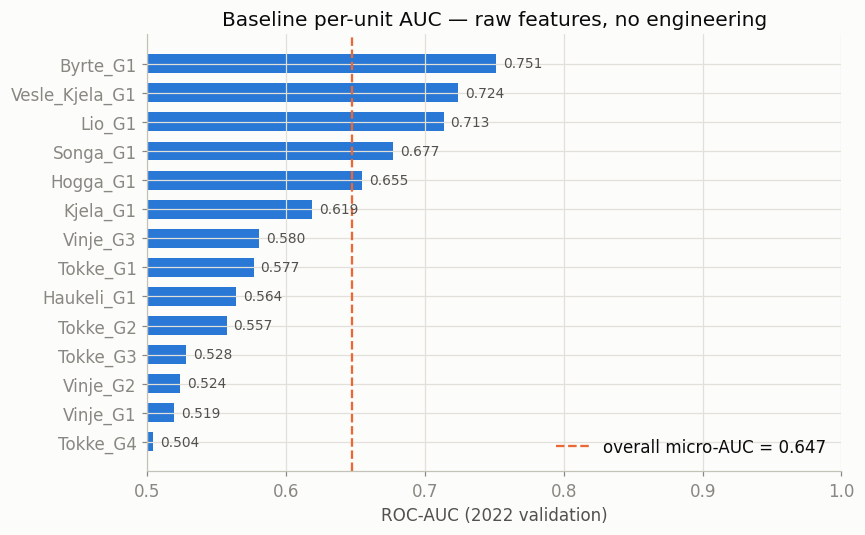
\includegraphics[width=0.75\linewidth]{figures/baseline_01_per_unit_auc.png}
  \caption{Per-unit AUC, baseline model, 2022 validation.}
  \label{fig:baseline-auc}
\end{figure}

\begin{figure}[htbp]
  \centering
  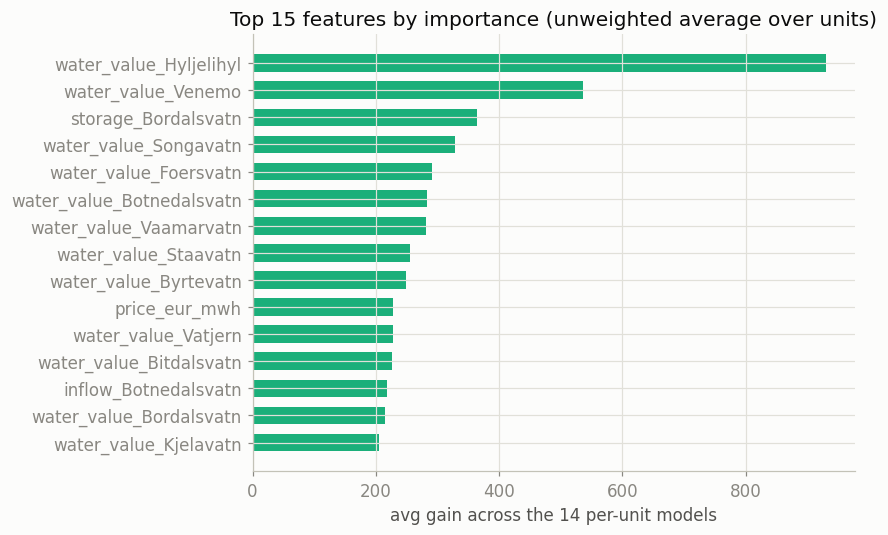
\includegraphics[width=0.75\linewidth]{figures/baseline_02_feature_importance.png}
  \caption{Top 15 features by average gain across the 14 per-unit models.}
  \label{fig:baseline-importance}
\end{figure}

\finding{Overall micro-AUC of 0.647 --- a workable but mediocre first baseline. Per-unit AUC
spans 0.50 (near-random, Tokke\_G4) to 0.75 (Byrte\_G1). The weakest units are almost exactly
the multi-unit Tokke (4 units) and Vinje (3 units) group --- the same units flagged as strongly
cross-correlated in Section~\ref{sec:eda}. Hypothesis (not yet tested): at a multi-unit plant,
\emph{how many} units are on may be easier to predict from price/water data than \emph{which
specific} unit(s), and 14 independent per-unit models have no way to share that information.}

\finding{Feature importance (Figure~\ref{fig:baseline-importance}) is smeared across many
similar reservoir columns rather than concentrated --- consistent with the observation that
every unit's model currently sees all 53 raw features (all 17 reservoirs), not just the ones
plausibly relevant to that unit's plant.}

This result (and every future one, scored the same way) is tracked in
\texttt{report/leaderboard.md} as it's produced, per \texttt{report\_rules.md}.
